\begin{frame}{Choosing the Right Comparable Area of Asia}
\vspace{-30pt}
    %\centering
\hspace{-30pt}
 \begin{minipage}{1.15\textwidth}
\begin{figure}[htb!]
    \centering
   \hspace{-40pt} 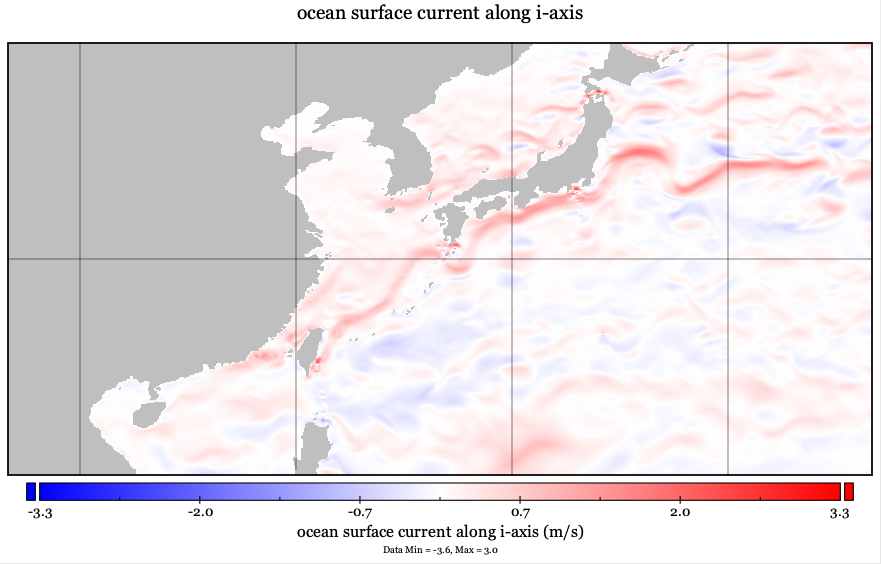
\includegraphics[width=0.42\linewidth]{images/example-images/c-uos.png}
        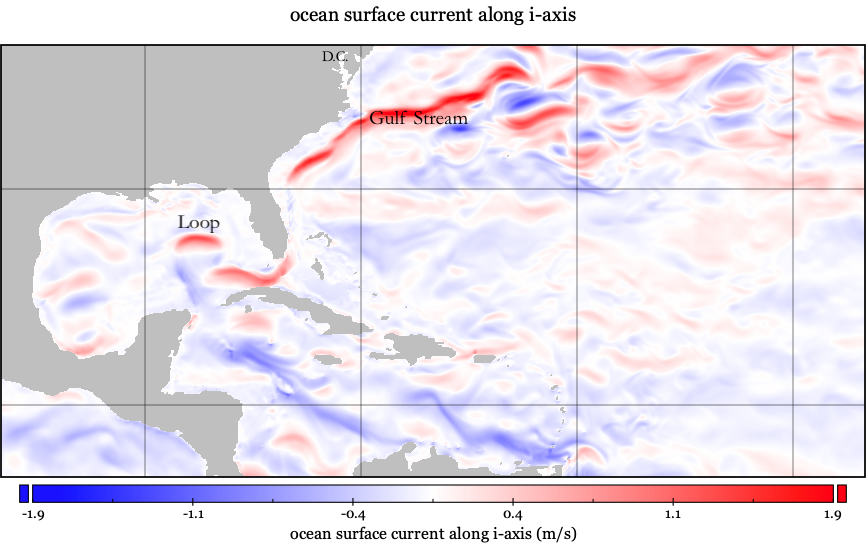
\includegraphics[width=0.42\linewidth]{images/example-images/uos.png}

   \hspace{-40pt} 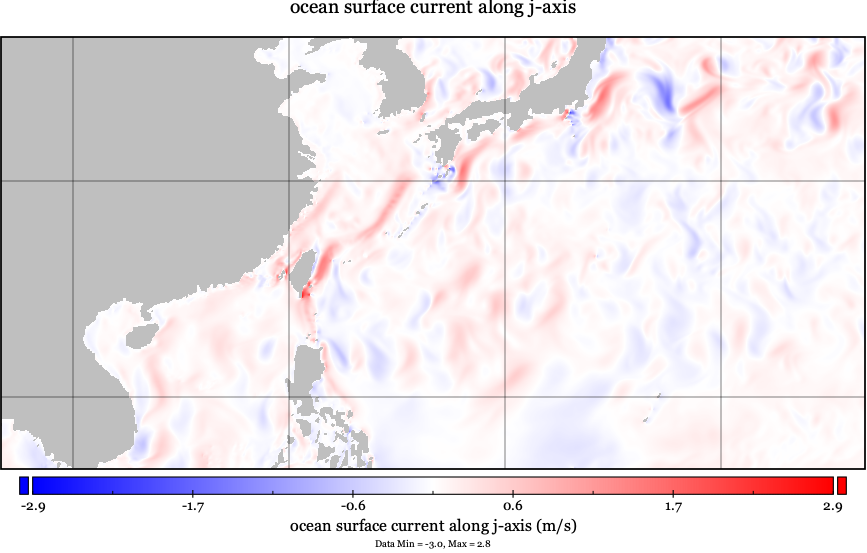
\includegraphics[width=0.42\linewidth]{images/example-images/c-vos.png}
        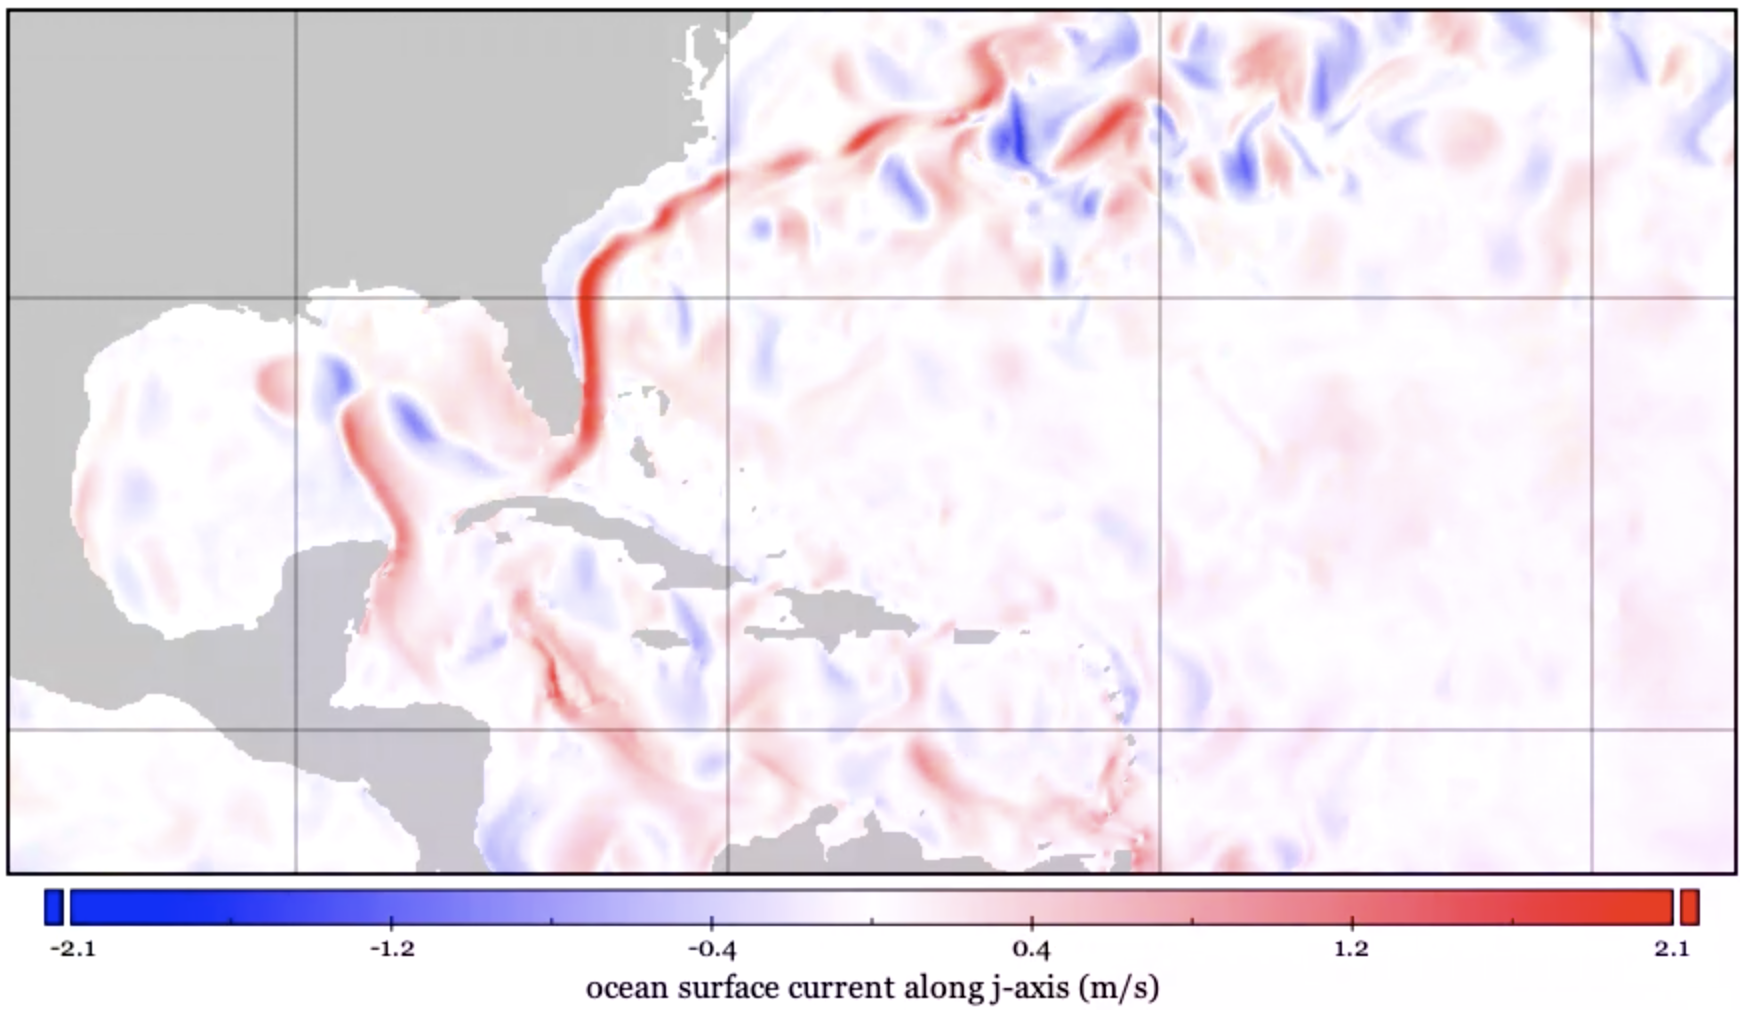
\includegraphics[width=0.42\linewidth]{images/example-images/vos.png}
    \vspace{-10pt}
    \caption{The Kuroshio and Gulf Stream share structural features.}
    \label{fig:A}
\end{figure}
\end{minipage}
\end{frame}


\begin{frame}{Helpful Coast Markers}
\vspace{-20pt}
    %\centering
 \begin{minipage}{1.0\textwidth}
\begin{figure}[htb!]
    \centering
    \includegraphics[width=1\linewidth]{../surge/plots/c_places.pdf}
    \vspace{-15pt}
   \caption{It might be useful to pick two coastal sections. }
    \label{fig:}
\end{figure}
\end{minipage}
\end{frame}
